\section{Introduzione}
L'obiettivo del rilievo è quello di descrivere quantitativamente il popolamento della pineta di Vallevecchia. I parametri dendrometrici interessati sono: il diametro medio, l'area basimetrica (totale o a ettaro), la distribuzione diametrica, l'altezza media, la curva ipsometrica e la stima del volume legnoso.

\textbf{Azienda Agricola di ValleVecchia}\\
Il sito in esame è localizzato all'interno dell'azienda agricola pilota "ValleVecchia" \ref{fig:veduta}, di proprietà della Regione Veneto e gestita da Veneto Agricoltura, all'interno del Comune di Caorle (Ve) \cite{veneto_agr}.\\
Nei quasi 800 ettari dell'azienda agricola, si possono trovare boschi planizali litoranei, siepi, zone umide, pinete e aree coltivate (per attività sperimentali).\\
Proprio per questo motivo, tra gli anni '50 e '60, è stata realizzata una pineta per difendere le colture dall'erosione del vento e del mare.\\
\textbf{La pineta}\\
La pineta analizzata in questo rilievo, pur non avendo importanti aspetti produttivi, oltre rappresentare un'importante difesa dal punto di vista idrogeologico, possiede una notevole funzione estetico-turistica nei confronti della spiaggia. \cite{tesi_rossetti}\\
Le due colture prevalenti presenti sono il pino domestico (Pinus pinea) e il pino marittimo (Pinus pinaster).\\
\textbf{Suolo}\\
Il suolo dell'azienda agricola presenta differenti composizioni chimiche, che possono essere suddivisi in tre differenti gruppi:
\begin{itemize}
    \item in bosco: prevalentemente sabbioso, con una grande quantità di calcio e magnesio, superiori agli altri siti;
    \item adiacenti ai corsi d'acqua: ricco di limo, argilla, sodio e zolfo;
    \item nelle produzioni colturali: alta percentuale di materia organica, azoto e fosforo.
\end{itemize}
Non sono state trovate rilevanti differenze nei suoli dei siti con diverse colture forestali \cite{tesi_paoletti}.\\
\textbf{Geografia e clima}\\
Essendo in una zona litoranea, l'altitudine dell'area d'interesse è di 0 m s.l.m.\\ All'interno dell'azienda agricola sono presenti dei canali d'acqua.\\
La temperatura media annua della zona, essendo di tipo sub-continentale, è di 12.6 °C; mentre le precipitazioni medie annue sono di 854 mm, distribuite secondo un regime pluviometrico sub-equinoziale \cite{grassland_in_a_changing_world}.\\
\begin{figure}
\centering
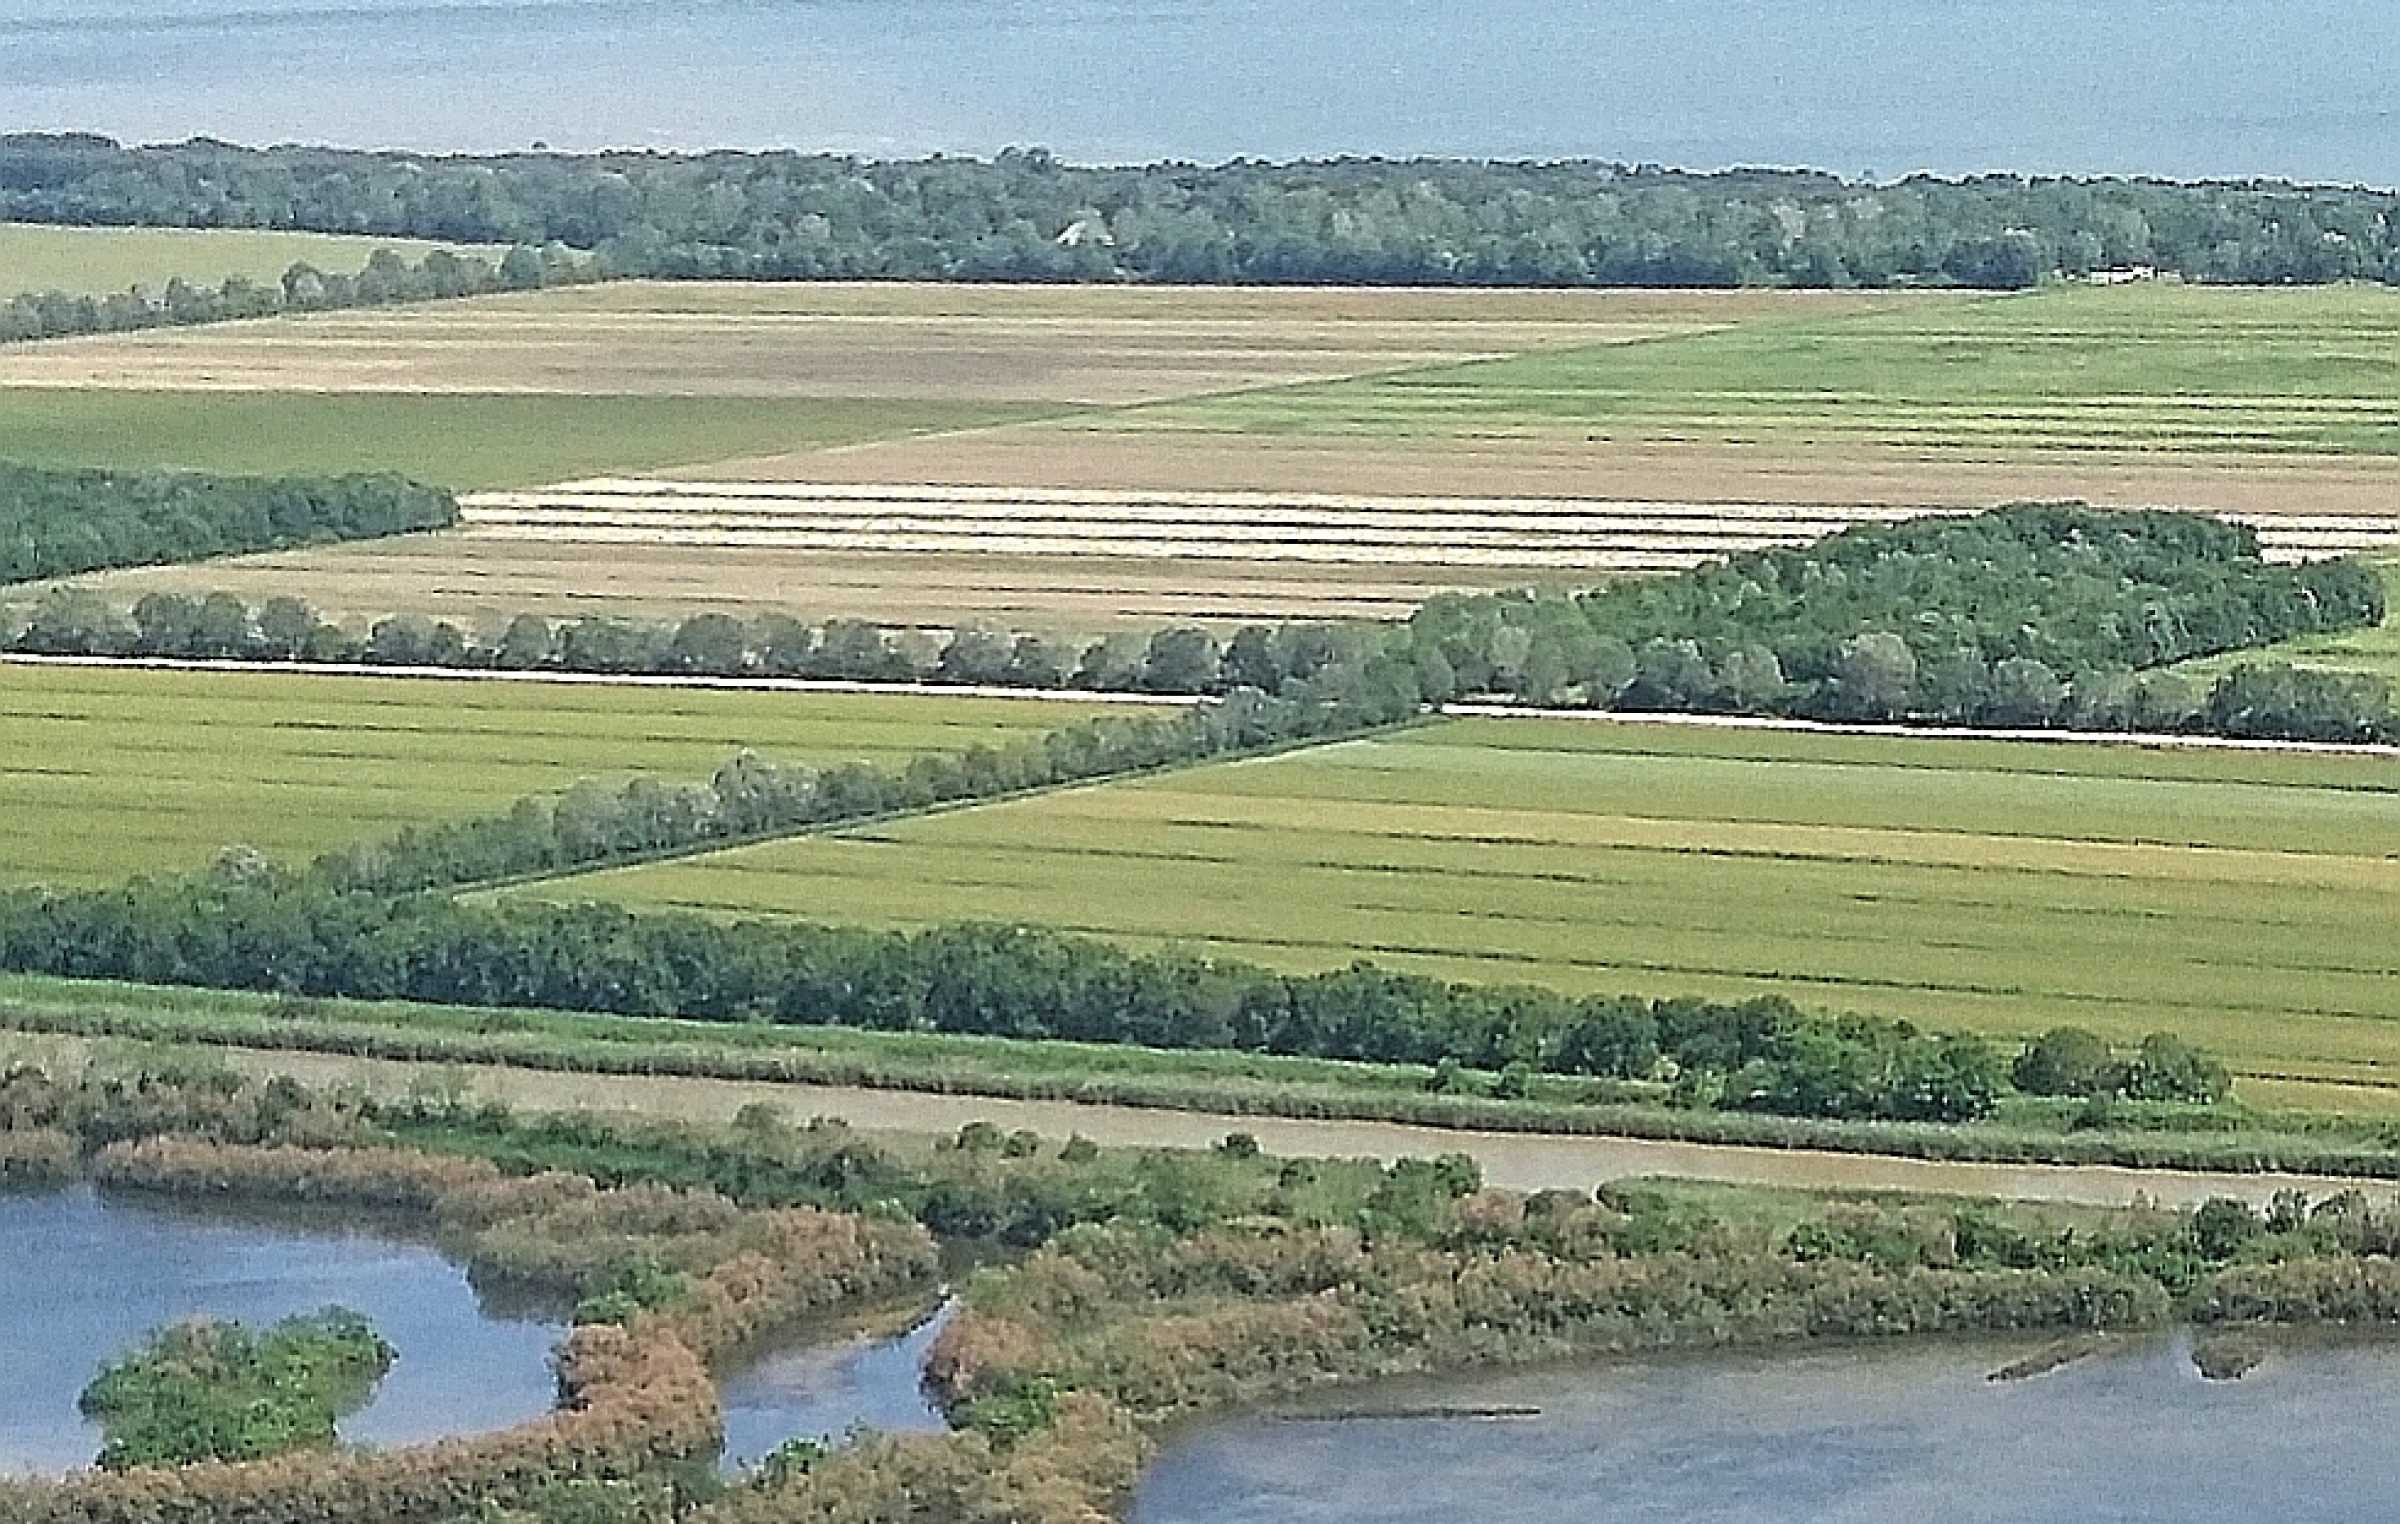
\includegraphics[width=6cm]{immagini/IMG_20190601_123742-2400x1524_c.jpg}
\caption{Veduta dell'azienda agricola Vallevecchia.}
\label{fig:veduta}
\end{figure}
 